\documentclass[12pt,a4paper,german]{report}
\usepackage{geometry}
\geometry{a4paper, top=25mm, left=25mm, right=25mm, bottom=30mm, headsep=10mm, footskip=12mm}
\usepackage[utf8]{inputenc}
\usepackage{titlesec}
\usepackage{blindtext}
\usepackage{hyperref}
\usepackage{babel}
\usepackage{titlepic}
\usepackage{graphicx}
\usepackage{algorithm}
\usepackage{amsmath}
\usepackage{mathptmx}
\usepackage{wrapfig}
\usepackage[onehalfspacing]{setspace}
\usepackage[noend]{algpseudocode}
\graphicspath{ {./images/} }

\titleformat{\chapter}{\normalfont\huge\bfseries}{\thechapter.}{20pt}{\huge\bfseries}

%%%%%%%%%%%%%%%%%%%%%%%%%%%%%%%%%%%%%%%%%%%%%%%%%%%%%%%%%%%%%%%%%%%%%%%%%%%%%%%%

\begin{document}

\begin{titlepage}
  \centering
  
\includegraphics[width=0.05\textwidth]{ktzh}\par
  {\scshape\LARGE Berufsmaturitätsschule Zürich \par}
  \vspace{0.25cm}
  {\scshape\Large Berufsmaturitätsarbeit \par}
  {\scshape Technik,  Architektur,  Life  Sciences \par}
  \vspace{0.50cm}
  {\huge\bfseries Pathfinding-Algorithmen: Einführung und Vergleich mittels einer Webapplikation \par}
  \vspace{0.5cm}
  Oberthema: \textsc{Mobilität} \\
  \vspace{0.5cm}
  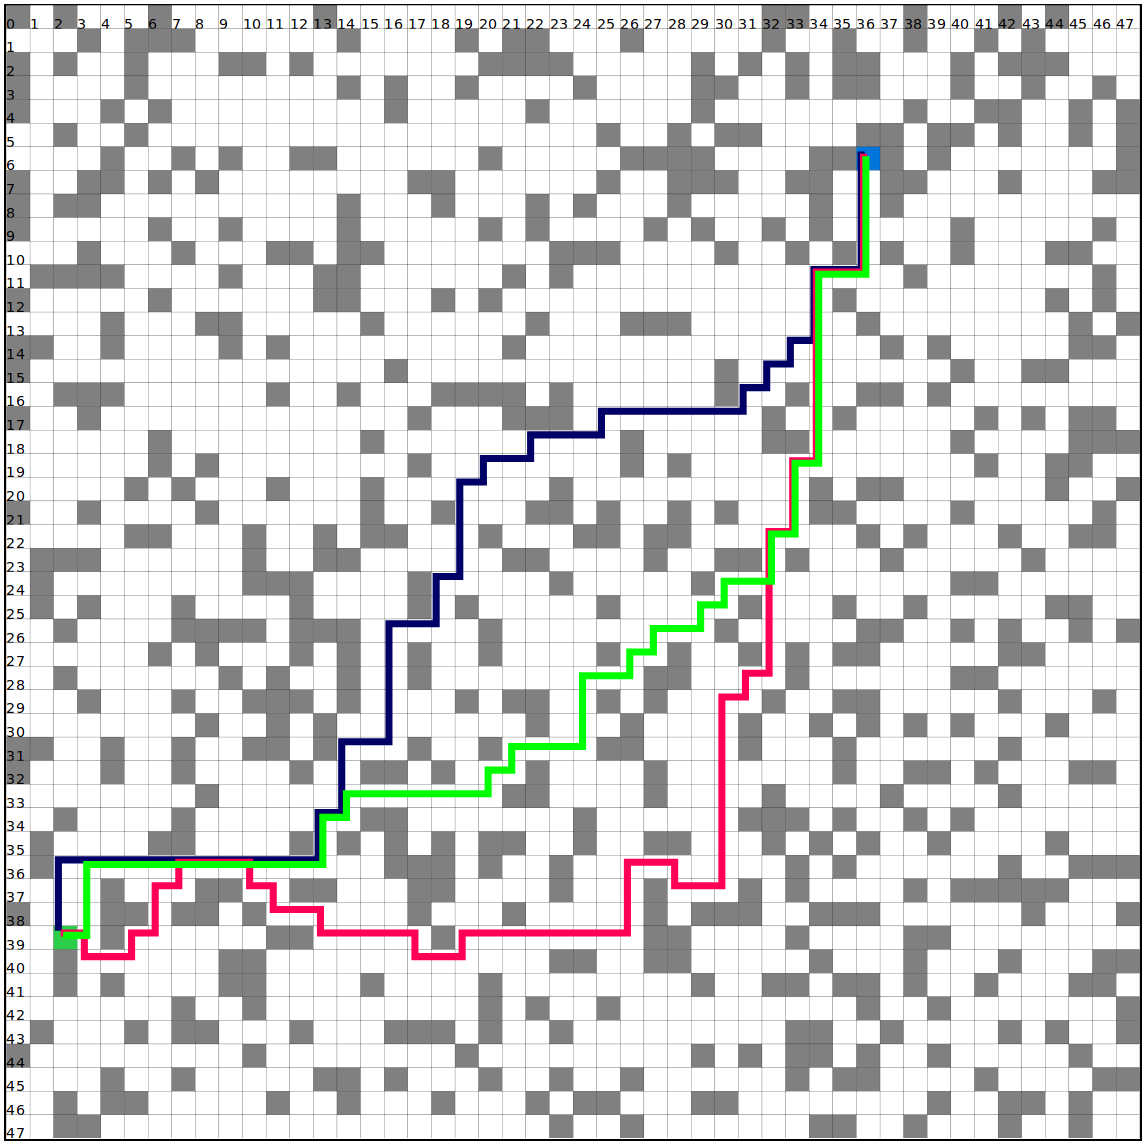
\includegraphics[width=0.65\textwidth]{cover2}\par
  \vspace{0.5cm}
  \begin{tabular}[t]{c@{\extracolsep{4em}}c} 
  \large\textsc{Adrian Stoop} & \large\textsc{Severin Fürbringer} \\ 
  adrian-stoop@gmx.ch & severin@fsfe.org\\
  EVT18a & EVT18a
  \end{tabular}
  \vfill
  \vspace{0.25cm}
  \large\textsc{Dr. Jürg Pöttinger}\\
  \normalsize{Begleitperson}
  \vspace{0.25cm}
  \vfill
  {1. Februar, 2019 \par}
\end{titlepage}


\renewcommand{\abstractname}{Abstract}
\begin{abstract}
Pathfinding-Algorithmen sind Programmabläufe, welche in der Wirtschaft in vielen Anwendungen vorkommen, wie zum Beispiel in Video Spielen, Simulationen oder der Automobilindustrie. 
Im Rahmen dieser Berufsmaturitätsarbeit wird eine Webapplikation entwickelt, die den Benutzer in das Thema der Pathfinder-Algorithmen einführt und einen interaktiven Vergleich von drei ausgewählten Pathfindern ermöglicht und dazu Messungen mit drei Merkmalen macht. Im Rahmen der Arbeit wählen wir den A*, BestFirst, und BreadthFirstFinder.
Die Webapplikation generiert für den Vergleich ein Zufallslabyrinth, markiert Start- und Endpünkte und lässt mehrere Vergleiche in Serie geschaltet zu.
Mithilfe des Pathfinder-Vergleichers werden im Rahmen der Arbeit auch Statistiken erstellt und ausgewertet und im schriftlichen Teil die Funktionsweisen der Pathfinder erläutert.
\\
  Die Webapplikation ist unter \url{https://bma.fuerbringer.info} zugänglich. Der dazugehörige Quellcode ist frei unter \url{https://github.com/fuerbringer/bma} erhältlich.
\end{abstract}


\tableofcontents{}

% START THESIS CONTENT
%%%%%%%%%%%%%%%%%%%%%%%%%%%%%%%%%%%%%%%%%%%%%%%%%%%%%%%%%%%%%%%%%%%%%%%%%%%%%%%%

\chapter{Einleitung}

%%%%%%%%%%%%%%%%%%%%%%%%%%%%%%%%%%%%%%%%%%%%%%%%%%%%%%%%%%%%%%%%%%%%%%%%%%%%%%%%
\chapter{Realisierung}
\section{Konzept}
Die Konzipierung dieser Webapplikation verlangte einige technische und gestalterische Entscheidungen. 
Einerseits musste die Programmiersprache und Struktur der Applikation geplant werden und andererseits auch das eigentliche Aussehen der Benutzeroberfläche der Webapplikation. 
Auf diese zwei wesentlichen Aspekte wird in diesem Abschnitt eingegangen.
\subsection{Pathfinding.js}
Eine korrekte Implementation der ausgewählten Pathfinder sind Voraussetzung für das Projekt. 
Daher wurde, um diese Voraussetzung zu erfüllen, eine frei verfügbare Implementation PathFinding.js \cite{pfjs} verschiedener Pathfinder ausgewählt.
\subsection{Programmierwerkzeuge}
Die vorhandenen Fachkenntnisse und Erfahrungen schlugen für die Implementierung entweder PHP oder JavaScript als mögliche Programmiersprachen vor. 
Zum Entscheid massgebend war, dass die Programmbibliothek PathFinding.js \cite{pfjs}, welche in unserer Arbeit eine wichtige Rolle spielt, in JavaScript implementiert wurde. 
Durch den Einsatz von JavaScript im Front-End und im Back-End, wäre es möglich die Pathfinder Berechnungen beliebig auf dem Rechner des Nutzers und auch auf dem Rechner des Servers auszuführen. 
Folgend werden die wichtigsten Technologien unserer Webapplikation aufgelistet\footnote{Eine komplette Auflistung inklusive der abhängenden Programmbibliotheken macht wenig Sinn, vor allem da unser Quellcode frei ersichtlich ist.}.

\begin{description}
  \item [Programmiersprache] JavaScript mit Einbindung von PathFinding.js \cite{pfjs}
  \item [Webserver-Software] Express\footnote{Express Webserver für Node Webapplikationen, \url{https://expressjs.com/}, Stand: \today}
  \item [Quellcode-Hosting] GitHub\footnote{GitHub, \url{https://github.com/}, Stand: \today}. Der Quellcode unser Webapplikation ist frei unter\\ \url{https://github.com/fuerbringer/bma} zugänglich.
  \item [Webhosting] Vultr\footnote{Vultr - The Infrastructure Cloud™, \url{https://vultr.com/}, Stand: \today}
\end{description}

\subsection{Konzipierung der Benutzeroberfläche}
Als Webapplikation muss unsere Arbeit deren Nutzen dem Benutzer ausreichend klar machen. 
Umsomehr ist dies von Bedeutung, da die Webapplikation frei zugänglich ist und daher auch Besucher den Sinn verstehen sollten. 
Aus diesem Grund wurde unsere Webapplikation für den Nutzer einführend gestaltet. 
Das heisst, dass der Benutzer beim Aufruf der Webapplikation zunächst auf einer Willkommensseite landet, die ihn wiederum zu einer Einführung in das Thema und Ziel der Arbeit führt. 
Nach der Einführung kann der Benutzer in der Visualisierung mit einzelnen Pathfindern erste Erfahrungen machen. 
Im Abschluss kommt der Benutzer zum Hauptteil der Arbeit, dem Pathfinding-Vergleicher. 
Ziel dieser Struktur ist, dass jede Person wenigstens einen Einblick in die Welt der Pathfinding-Algorithmen erhält.
\begin{figure}[h]
  \centering
  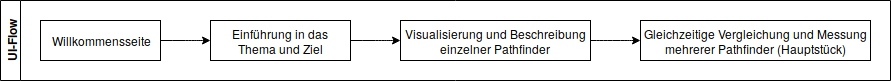
\includegraphics[width=16cm]{uiflow}
  \caption[Struktur der Webapplikation.]{Webapplikationsstruktur. Quelle: Eigenleistung}
  \label{fig:uiflow}
\end{figure}

\clearpage

\subsubsection{Einführungs- und Willkommensseite}
Die Einführungsseite erklärt dem Benutzer was Algorithmen sind und führt ihn anschliessend mit einfachen Beispielen in das Thema Pathfinder ein. Zuletzt werden die Ziele der Arbeit aufgelistet.
\begin{figure}[h]
  \centering
  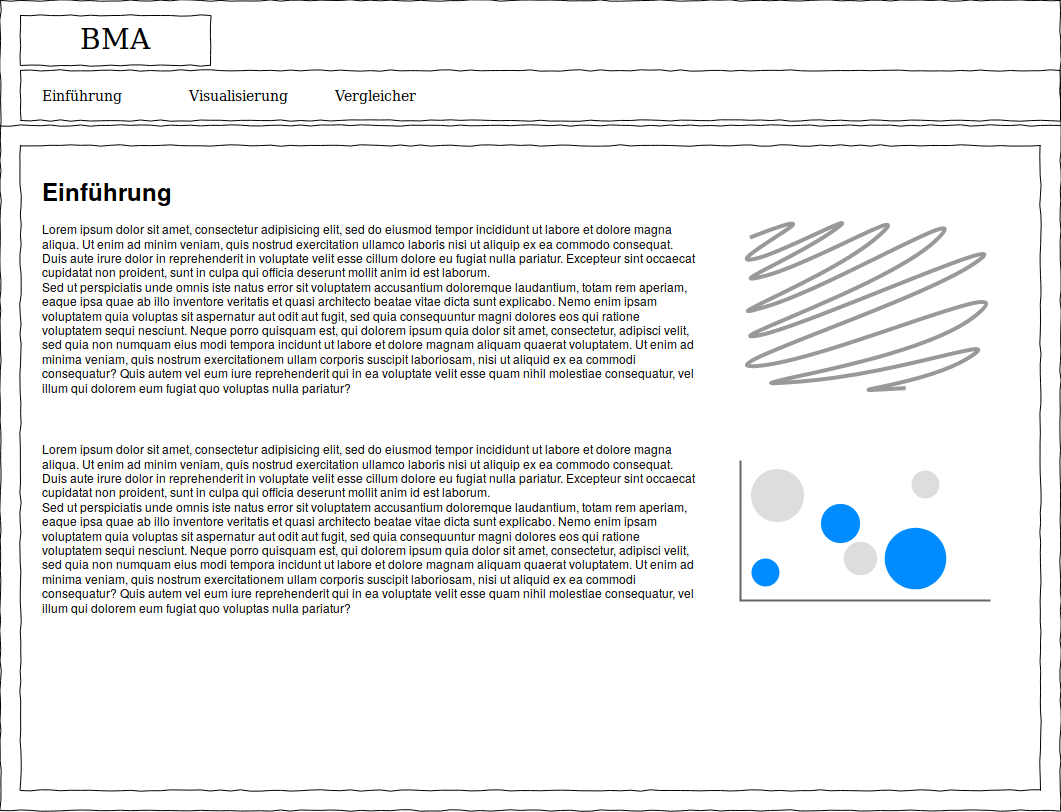
\includegraphics[width=16cm]{einfuehrung1}
  \caption[Konzept der Einführungsseite.]{Einführungsseite. Quelle: Eigenleistung}
  \label{fig:einfuehrung1}
\end{figure}

\clearpage

\subsubsection{Visualisierung der Pathfinder}
Nach der Einführung erhält der Benutzer die Möglichkeit mit einzelnen Pathfindern zu experimentieren. Dazu kann er auch verschiedene Parameter anpassen. Dies ist die Vorstufe zum Pathfinder-Vergleicher, da hier nochmals die einzelnen Pathfinder auf ihre Eigenschaften beschrieben werden.
\begin{figure}[h]
  \centering
  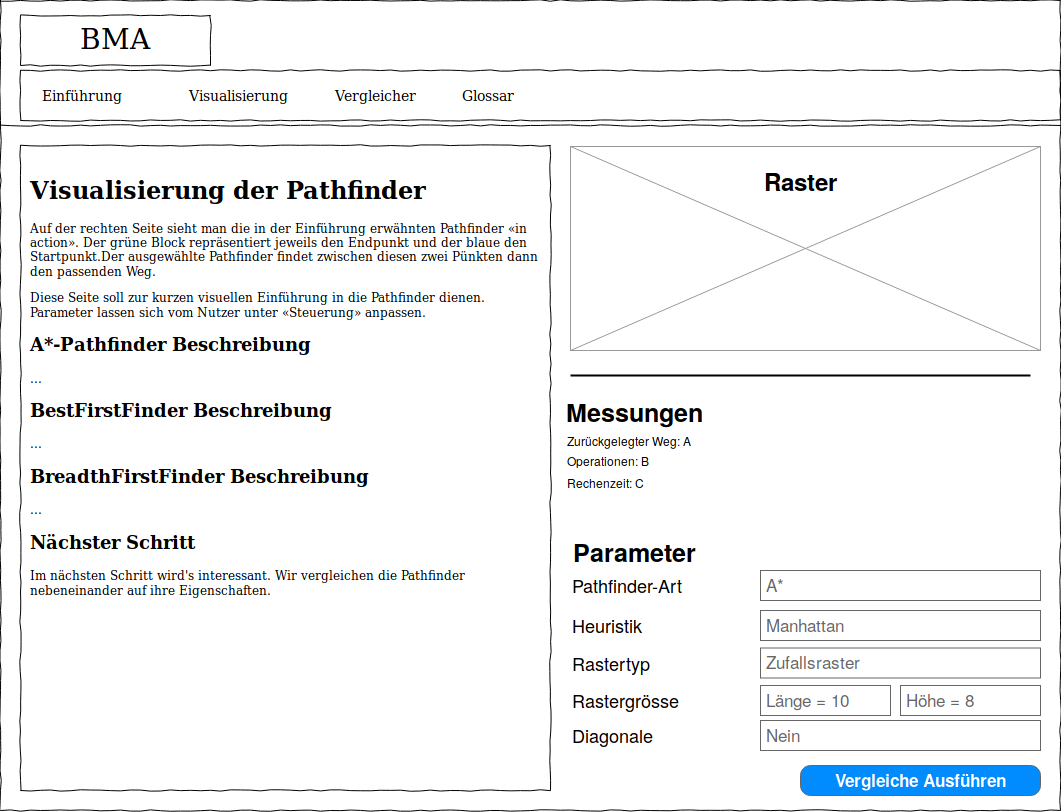
\includegraphics[width=16cm]{visualisierung1}
  \caption[Benutzeroberflächenkonzept des Pathfinding-Visualisierers.]{Benutzeroberflächenkonzept Visualisierer. Quelle: Eigenleistung}
  \label{fig:gui_konzept_visualizer}
\end{figure}

\clearpage

\subsubsection{Vergleich der Pathfinder}
Als Herzstück der Arbeit ermöglicht der Pathfinder-Vergleicher dem Nutzer die ausgewählten Pathfinder zu vergleichen. Hier werden, gleich wie beim Visualisierer, zuerst vom Benutzer die Parameter gewählt. Die parallel ausgeführten Resultate mit Informationen über die Rechenzeit, zurückgelegten Weg und Operationen, sind dann interaktiv anwählbar. Gleichzeitig wird auch unter ``Resultate'' unten links das Total aller Vergleiche akkumuliert, damit ein Gesamteindruck verschaffen werden kann.

\begin{figure}[h]
  \centering
  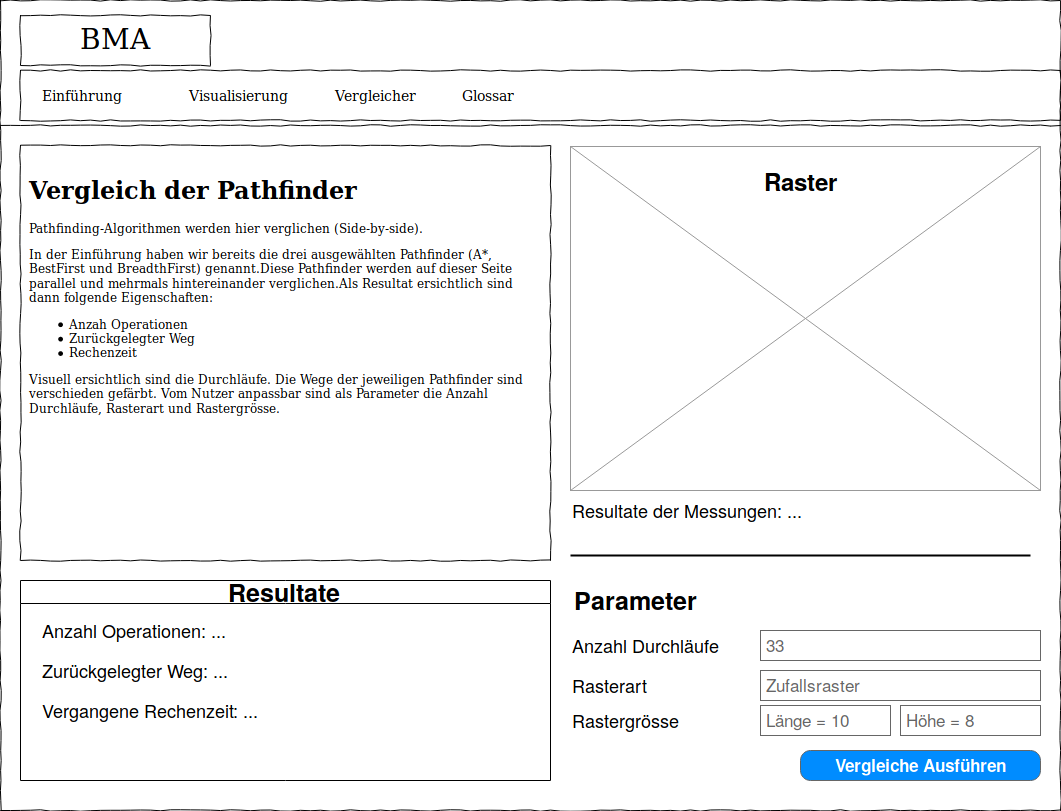
\includegraphics[width=16cm]{konzept1}
  \caption[Benutzeroberflächenkonzept des Pathfinder-Vergleichers.]{Benutzeroberflächenkonzept Vergleicher. Quelle: Eigenleistung}
  \label{fig:gui_konzept_comparator}
\end{figure}

\section{Implementierung des Vergleichers}
Vor allem für die statistischen Auswertungen ist es von Bedeutung zu wissen, wie der Vergleicher zu den Resultaten kommt und die Berechnungen durchführt. Um an die statistischen Merkmale zu gelangen, musste je nach Merkmal die Webapplikation oder PathFinding.js erweitert werden.

\subsection{Zurückgelegter Weg}
Der zurückgelegte Weg ist aus praktischer Sicht gesehen ein bedeutendes Merkmal, da man möchte, dass der resultierende Weg möglichst kurz ausfällt. 
Die Programmbibliothek PathFinding.js liefert den Weg in einer Liste mit einer Koordinate pro Element. 
Daraus folgt, dass der Weg $s$ der Anzahl der Elemente der Liste entsprechen muss, wenn man nach PathFinding.js Sprünge oder Luftlinien ausschliest\footnote{Ein von PathFinding.js berechneter Weg: \url{https://pathfindingjs.readthedocs.io/en/latest/user-guide/getting-started/}}. 
Es gibt demnach keine Geraden, ausser zwischen zwei Benachbarten Pünkten.
Diagonalen würden nach dieser Logik bei einem diagonalen Sprung als eine Wegeinheit gelten.
\[ s = n
\begin{cases}
  P_1(0,0)\\
  P_2(1,0)\\
  ...\\
  P_n(11,4)
\end{cases}
\]
\subsection{Operationen}
Ein Algorithmus, der für das gleiche Resultat weniger Schritte (Operationen) tätigen muss, ist grundsätzlich besser als ein anderer, solange die Rechenzeit ebenfalls kleiner ausfällt. Für das wichtige Nebenmerkmal zur Rechenzeit mussten die internen Routinen der Programmbibliothek PathFinding.js angepasst werden, da sie solche Messungsmerkmale nicht standardmässig liefert. Dazu wurde das PathFinding.js kopiert und in die Routinen der drei ausgewählten Pathfinder im äusseren und inneren Loop eingefügt. Folgende Dateien\footnote{Die genauen Anpassungen sind unter dem folgenden Link verfügbar: \url{https://github.com/fuerbringer/PathFinding.js/commit/51034158638ad7aaa9c5142a827bd4d3de2b8786\#diff-22360b18a43ac33ae398e44b998101c7}} wurden dafür angepasst:
{Rechenzeit}
\begin{itemize}
\item{src/finders/AStarFinder.js}
\item{src/finders/BreadthFirstFinder.js}
\end{itemize}
Zu beachten ist, dass die Datei des BestFirstFinders nicht angepasst werden musste, da dieser auf dem A*-Finder basiert und somit alle Änderungen vom A*-Finder vererbt.

\subsection{Rechenzeit}
Ein bedeutendes Merkmal ist die Rechenzeit, also die Zeit, in der der Pathfinder seine Arbeit verrichtet hat. 
Um diese zu berechnen, wird unmittelbar vor der Ausführung der Wegfindungsroutine des Pathfinders der Zeitstempel $t_0$ der jetzigen Zeit zwischengespeichert und danach vom Pathfinder die Arbeit verrichtet. 
Direkt nach dem Beenden der Wegfindung wird ein zweites Mal ein Zeitstempel $t_1$ zwischengespeichert. Die Differenz ergibt die Zeit $t$ in Millisekunden\footnote{Die Einheit Millisekunden ergibt sich aus der Schnittstelle \texttt{Performance.now()} von JavaScript}, die für die Berechnung benötigt wurde.
\begin{equation}
  t = t_1 - t_0
\end{equation}
Die Werte $t$ sind pro Pathfinder in der Webapplikation unter ``Messung für diesen Einzelversuch:'' unter dem Raster ersichtlich. Diese Berechnung demnach pro Durchlauf dreimal getätigt.
\\\\
Aus diesen drei Merkmalen folgen zusammengefasst die in unserer Webapplikation vermessenen Werte der Pathfinding-Algorithmen.
\begin{figure}[h]
  \centering
  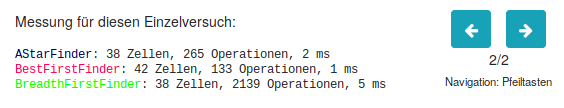
\includegraphics[width=10cm]{measurements_single}
  \caption[Ausschnitt aus dem Pathfinding-Vergleicher für einzelne Vergleiche.]{Vergleicherausschnitt. Quelle: Eigenleistung}
  \label{fig:gui_konzept_comparator}
\end{figure}


%%%%%%%%%%%%%%%%%%%%%%%%%%%%%%%%%%%%%%%%%%%%%%%%%%%%%%%%%%%%%%%%%%%%%%%%%%%%%%%%
\chapter{Schluss}
\blindtext

\chapter{Glossar}
\section*{Fachwörter- und Begriffsverzeichnis}
In diesem Kapitel werden wichtige Wörter aus der Fachsprache erklärt, die in unserer Arbeit oftmals vorkommen.
\paragraph{A*} Sprich ``A Star''. Ein Pathfinding Algorithmus (siehe Fachbegriff Algorithmus). Dieser nutzt zusätzlich heuristische Mittel, um den Weg zu berechnen (siehe Heuristik).
\paragraph{Algorithmus} Ein Ablauf, Prozess oder Programm, der eine Liste mit Anweisungen schrittweise befolgt, um Daten umzuwandeln.
\paragraph{Back-End} Der Server---mit guten Systemtechnikern rund um die Uhr stellt das Back-End die Website unter einer URL, wie \texttt{bma.fuerbringer.info}, zur Verfügung.
\paragraph{BestFirstFinder} Ein Pathfinding-Algorithmus. Nicht zu verwechseln mit dem BreadthFirstFinder.
\paragraph{BreadthFirstFinder} Ein Pathfinding-Algorithmus. Nicht zu verwechseln mit dem BreadthFirstFinder.
\paragraph{Dijkstra} Ein Pathfinding Algorithmus (siehe Fachbegriff Algorithmus). Dieser nutzt keine heuristische Mittel und kommt in unserer Arbeit nicht direkt vor.
\paragraph{Front-End} Der Browser---der Teil einer Website oder Webapplikation, den der Benutzer sieht und mit dem er interagiert. In unserem Fall werden die wichtigsten Berechnungen im Front-End verrichtet.
\paragraph{Heuristik} Hilfsalgorithmus, unter Anderem für Pathfinder, der zusätzlich hilft zwischen einzelnen Schritten die Kosten für eine mögliche Operation einzuschätzen.
\paragraph{Matrix} Anordnung von Elementen. In unserem Fall ein zweidimensionales Raster, in dem Wände, Korridore und Wege platziert sind.
\paragraph{Operationen} Eine ``Operation'' beschreibt in unserem Fall einen Zyklus eines Pathfinders. Je mehr Zyklen ein Pathfinder in Relation zu einem anderen benötigt, desto weniger effizient ist er.
\paragraph{Parameter} Die Randbedingungen für einen Durchlauf bzw. ein Experiment.
\paragraph{PathFinding.js} Die Zentrale Programmbibliothek, deren Pathfinder Implementationen wir in unserer Webapplikation nutzen.
\paragraph{Pathfinder} Eine Art Algorithmus, der in einem gegebenen Raum mit eingezeichnetem Start- und Endpunkt den schnellsten weg Findet.
\paragraph{recbacktracker} ``Recursive Backtracker, ein Labyrinthalgorithmus, den wir in unserer Webapplikation zur Generierung von perfekten (immer lösbaren) Labyrinthen verwenden. Dieser Algorithmus kommt im Vergleicher nicht zum Zug.


% TODO
% Danksagung

% END THESIS CONTENT
%%%%%%%%%%%%%%%%%%%%%%%%%%%%%%%%%%%%%%%%%%%%%%%%%%%%%%%%%%%%%%%%%%%%%%%%%%%%%%%%

\clearpage

\begin{thebibliography}{9}
\bibitem{pfjs}
  Xueqiao Xu et al.,
  \textit{PathFinding.js},
  \url{https://github.com/qiao/PathFinding.js},
  Quellcode auf GitHub,
  Letzter Aufruf: \today
\bibitem{cuishi2011}
  Xiao, Cui; Hao Shi,
  \textit{A*-based Pathfinding in Modern Computer Games},
  IJCSNS International Journal of Computer Science and Network Security, VOL.11 No.1,
  Januar 2011.
\bibitem{bma}
  Fürbringer, Severin; Stoop, Adrian,
  \textit{BMA Quellcode},
  \url{https://github.com/fuerbringer/bma},
  \today
\bibitem{bmaonline}
  Fürbringer, Severin; Stoop, Adrian,
  \textit{BMA-Webapplikation},
  \url{https://bma.fuerbringer.info},
  \today
\end{thebibliography}


\listoffigures

\end{document}
